\documentclass{beamer}[10pt, usepdftitle=false, handout]

\beamertemplatenavigationsymbolsempty

\usepackage[T1]{fontenc}
\usepackage[]{algorithm2e}
\usepackage{multimedia}
\usepackage{gensymb}
\usepackage{textcomp}
%\usepackage{background}
%\backgroundsetup{
%    placement=center,
%    scale=1,
%    contents={The author of this course is PAUL BLONDEL},
%    opacity=0.7
%}
%\setbeamertemplate{background}{\BgMaterial}

%\usepackage[font=small,labelfont=bf]{caption} 

\usetheme{Boadilla}

\title{Data Structure 2}
\author[]{Paul Blondel}
\institute[]{CNAM}
\date[]{September 1st, 2018}

\usepackage[style=british]{csquotes}


\def\signed #1{{\leavevmode\unskip\nobreak\hfil\penalty50\hskip1em
  \hbox{}\nobreak\hfill #1%
  \parfillskip=0pt \finalhyphendemerits=0 \endgraf}}

\newsavebox\mybox
\newenvironment{aquote}[1]
  {\savebox\mybox{#1}\begin{quote}\openautoquote\hspace*{-.7ex}}
  {\unskip\closeautoquote\vspace*{1mm}\signed{\usebox\mybox}\end{quote}}


%\setbeamertemplate{headline}
%{
%  \leavevmode%
%  \hbox{%
%  \begin{beamercolorbox}[wd=1.0\paperwidth,ht=2.25ex,dp=1ex,center]{author in head/foot}%
%   \textcolor{green}{- This course has been made by Paul Blondel -} \usebeamerfont{author in head/foot}\insertsubsection
%  \end{beamercolorbox}}%
%  \vskip0pt%
%}


\setbeamertemplate{footline}
{
  \leavevmode%
  \hbox{%
  \begin{beamercolorbox}[wd=.5\paperwidth,ht=2.25ex,dp=1ex,center]{author in head/foot}%
    \usebeamerfont{author in head/foot}\insertsection
  \end{beamercolorbox}%
  \begin{beamercolorbox}[wd=.5\paperwidth,ht=2.25ex,dp=1ex,center]{title in head/foot}%
    \usebeamerfont{title in head/foot} \inserttitle \hspace*{2em}  \insertframenumber{} / \inserttotalframenumber\hspace*{2ex} 
  \end{beamercolorbox}}%
  \vskip0pt%
}

\AtBeginSection[]
{
   \begin{frame}
    \tableofcontents[ 
    currentsection,hideallsubsections] 
   \end{frame}
}

\begin{document}
	{
	\setbeamertemplate{footline}{
  	\leavevmode%
  	\hbox{%
  	\begin{beamercolorbox}[wd=.5\paperwidth,ht=2.25ex,dp=1ex,center]{author in head/foot}%
  	\end{beamercolorbox}%
  	\begin{beamercolorbox}[wd=.5\paperwidth,ht=2.25ex,dp=1ex,center]{title in head/foot}%
  	\end{beamercolorbox}}%
  	\vskip0pt%	
	} 
	\begin{frame}
	\titlepage
	\end{frame}

	\begin{frame}
	
	\begin{aquote}{Linus Torvalds}
	I will, in fact, claim that the difference between a bad programmer and a good one is whether he 
	considers his code or his data structures more important. Bad programmers worry about the code. Good programmers worry about data structures and their relationships.	
	\end{aquote}	
	
	\end{frame}


	\begin{frame}
		\tableofcontents[hideallsubsections]
	\end{frame}
	}

	\addtocounter{framenumber}{-3}

	\section{Sequential data structures}	
	\subsection{First notions}	

    \begin{frame}[label=(first)]
    
	\begin{block}{What is a data structure?}
	A data structure is a \textbf{set of variables} of the \textbf{same nature}
	\end{block}
		
	\vspace*{1em}		

	A variable of a data structure can be accessed ...
	
	\begin{itemize}
	\item {... either directly by \textbf{giving a specific index} (a number)}
	\item {... or by \textbf{traversing the structure in order}}
	\item {... sometimes by \textbf{both methods} (directly and by traversing)}
	\end{itemize}
			

		
	\end{frame}
	
	\subsection{Different types of sequential data structure}			
	
	\begin{frame}	
	
	There are three types of sequential data structures:
	
	\begin{enumerate}
	\item {\textbf{contiguous} data structure
		\begin{itemize}
			\item {Arrays}
			\item {Sequential files}
		\end{itemize} }	
	\item {\textbf{linked} data structure
		\begin{itemize}
			\item {linked-list}
		\end{itemize} }
	\item {\textbf{abstract} data structure 
		\begin{itemize}
			\item {Stacks}
			\item {Queues} 
		\end{itemize}	
	}		
	\end{enumerate}
	
	
	\end{frame}
	
	\section{Contiguous data structure - Arrays}
	\subsection{Properties}	
	
	\begin{frame}
	
	\begin{exampleblock}{Contiguous?}
	Array are said contiguous because all their \textbf{variables are contiguously stored in memory} (= variables stored one after the other in memory).
	\end{exampleblock}	
	
	\pause	
	
	For instance, let's draw an empty array of size $N$:
	
			
	\begin{figure}
	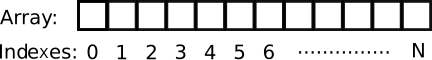
\includegraphics{images/array_01.png} 
     	%\vspace*{-0.5em}
		%\caption{Floating gate transistor cell}
		\end{figure}		
	%	sasasasa
	\pause	
	
	Let's now draw an array of characters containing "HELLO DONGGUAN":
	
	\begin{figure}
		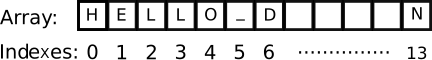
\includegraphics{images/array_02.png} 
     	%\vspace*{-0.5em}
		%\caption{Floating gate transistor cell}
	\end{figure}

	To access a specific variable just specify the index, example: Array[3] == L, to access the next variable I just increase the index: Array[4] == O, and so on.
	
	\end{frame}
	
	\begin{frame}
	
	Examples of two basic array usage in pseudo-code:
	
	\begin{center}    
    \scalebox{0.75} {
    %\begin{minipage}
    \begin{algorithm}[H]
	i = 0\; 	
 	\While{i < N}{
 	  AnyFunction(Array[i])\;
	  i=i+1\;
	}
 	\caption{Traversing an array, index after index...}
	\end{algorithm}	
	%\end{minipage}
	}
	\end{center}    
	

    \begin{center}    
    \scalebox{0.75} {
    %\begin{minipage}
    \begin{algorithm}[H]
	i = 0\; 
	Sum = 0\;	
 	\While{i < N}{
 		Sum = Sum + Array[i]\;
		i=i+1\;
	}
 	\caption{Sum of array elements}
	\end{algorithm}	
	%\end{minipage}
	}
	\end{center}    
	
	\end{frame}	
	
	\subsection{Searching an element}		
	
	\begin{frame}	
			
	First, let's assume our array contains a list of \textbf{non-sorted elements}\footnote{sorted list of elements: 1 ,4 ,7 , 20, 55, non-sorted list of elements: 7, 5, 1, 2, 10}.

	\begin{figure}
		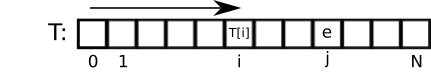
\includegraphics[scale=0.8]{images/array_03.png} 
     	%\vspace*{-0.5em}
		%\caption{Floating gate transistor cell}
	\end{figure}
	
	\vspace*{-1.0em}
	
	\pause
	
	To search and find the "e" value in $T$ we can perform a \textbf{sequential search}:
	
	\begin{center}    
    \scalebox{0.75} {
    %\begin{minipage}
    \begin{algorithm}[H]
	i = 0\; 
 	\While{i <= N and T[i] != e}{
 		i=i+1\;
	}
 	%\caption{Sequential search through the array}
	\end{algorithm}	
	%\end{minipage}
	}
	\end{center}    
	
	\pause
	
	Here we have the following complexities:
	
	\begin{itemize}
	\item {at best: 1}
	\item {at worst: N}
	\item {in average: $\frac{N}{2}$ (\textbf{if e belongs to T!})}	
	\end{itemize}			
		
	\end{frame}

	\begin{frame}
	
	First, let's now assume our array contains a list of \textbf{sorted elements}.
	
	\begin{figure}
		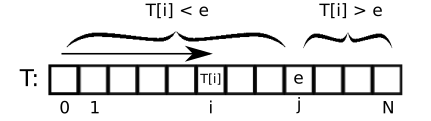
\includegraphics[scale=0.8]{images/array_04.png} 
     	%\vspace*{-0.5em}
		%\caption{Floating gate transistor cell}
	\end{figure}
	
	\vspace*{-1.0em}
		
	\pause
	
	Now that the array is sorted, the \textbf{sequential search} is slightly different:
	
	\begin{center}    
    \scalebox{0.75} {
    %\begin{minipage}
    \begin{algorithm}[H]
	i = 0\; 
 	\While{i <= N and T[i] < e}{
 		i=i+1\;
	}
 	%\caption{Sequential search through the array}
	\end{algorithm}	
	%\end{minipage}
	}
	\end{center}
	
	\pause
	
	This time we have the following complexities:
	
	\begin{itemize}
	\item {at best: 1}
	\item {at worst: N}
	\item {in average: $\frac{N}{2}$ (\textbf{if e belongs \textit{or NOT} to T})}	
	\end{itemize}	
	
	\end{frame}

	\begin{frame}
	
	Let's now perform a \textbf{dichotomic search} on a sorted array:
	
	\begin{figure}
		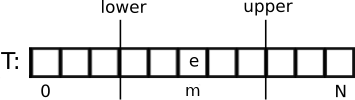
\includegraphics[scale=0.8]{images/array_05.png} 
     	%\vspace*{-0.5em}
		%\caption{Floating gate transistor cell}
	\end{figure}
	
	%\vspace*{-1.0em}
	%\pause
	
	The $upper$ and $lower$ boundaries are adjusted step by step until finding "e":
	
	\begin{columns}[c]
	\column{.5\textwidth} 
	\begin{center}    
    \scalebox{0.75} {
    %\begin{minipage}
    \begin{algorithm}[H]
	lower = 0; upper = N\; found=False; m=0\; 
 	\While{lower<=upper and found == False}{
 		m=(lower+upper) / 2\;
 		
		\eIf{T[m]==e} {
			found=True
		} {
			\eIf{T[m]<e} {
				lower=m+1\;
			} {
				upper=m-1\;
			}		
		}	 		
	}
 	%\caption{Sequential search through the array}
	\end{algorithm}	
	%\end{minipage}
	}
	\end{center}			
	
	\column{.5\textwidth}
	\begin{center}
	Here we have these complexities:
	\begin{itemize}
	\item {at best: 1}
	\item {at worst: $log_2(N)$}	
	\end{itemize}		
		
	\end{center}	
		
	\end{columns}
	
	\end{frame}
	
	\subsection{Inserting an element}
	
	\begin{frame}
	
	%\begin{block}{How do I add new values to my array?}
	%By inserting new values to the sequential structure!
	%\end{block}
	How inserting new values to my array?
		
	%\vspace*{-0.5em}	
	
		\begin{figure}
		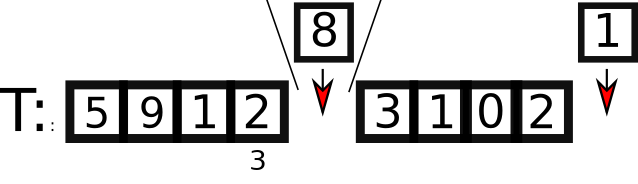
\includegraphics[scale=0.4]{images/array_06.png} 
     	%\vspace*{-0.5em}
		%\caption{Floating gate transistor cell}
	\end{figure}	
	
	%\vspace*{-0.5em}	
	
	If your array is \textbf{NOT sorted} ...		
	
	\begin{itemize} 
		\item {... you can insert the element \textbf{at the end} (by default)}
		\item {or you can \textbf{specify after which index} you want to insert (ex: 3)}		
	\end{itemize}	
	
	\pause
	
	%\vspace*{-0.5em}
	
	\begin{figure}
		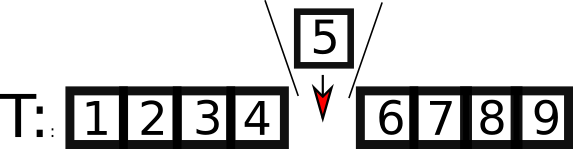
\includegraphics[scale=0.4]{images/array_07.png} 
     	%\vspace*{-0.5em}
		%\caption{Floating gate transistor cell}
	\end{figure}		
	
	%\vspace*{-0.5em}	
	
	If your array is \textbf{sorted} ...	
	
	\begin{itemize}
		\item {... your insert should respect the \textbf{sorting order}!\footnote{Not doing this would make your array unsorted.}}	
	\end{itemize}
		
	
	\end{frame}

	\begin{frame}
	
	Let's assume inserting at the end of a \textbf{non-sorted} array is evident.	 

	\vspace*{1em}	
	Now, for inserting an element in a specific position "pos", let's do:\
	\begin{columns}[c]
	\column{.5\textwidth}
	\begin{center}    
    \scalebox{0.75} {
    %\begin{minipage}
    \begin{algorithm}[H]
    reallocate\_memory\_and\_copy(T)\;
	i=pos\;
 	\While{i < N}{
		T[i+1] = T[i]\;
		i=i+1\;
	}
	N=N+1\;
	T[pos]=e\;
 	%\caption{InnserSequential search through the array}
	\end{algorithm}
	%\end{minipage}
	}
	\end{center}	
	\column{.5\textwidth}
	\begin{center}
	
	Here we have these complexities:
		
	\begin{itemize}
	\item {at best: 1}
	\item {at worst: N}
	\item {in average: $\frac{N}{2}$}	
	\end{itemize}		
	
	\end{center}
	\end{columns}	
	
	\pause
	
	\vspace*{1em}
	
	\begin{alertblock}{Note}
	\begin{itemize}
	\item {Inserting at the end is only $O(1)$, this should be preferred!}
	\item {The size of $T$ has to be increased by 1 (for the new value)}
	\end{itemize}
	\end{alertblock}		
	
	\begin{block}{Note}
	In the next slides, this "insert" function will call the pseudo-code above
	\end{block}
	
	\end{frame}
	
	\begin{frame}
	
	Inserting a new value "e" in a \textbf{sorted array} requires a different approach:
	
	\begin{columns}[c]
	\column{.5\textwidth}
	\begin{center}    
    \scalebox{0.75} {
    %\begin{minipage}
    \begin{algorithm}[H]
    reallocate\_memory\_and\_copy(T)\;
    // search part below\\
    i=0;pos=0\;
 	\While{i<N and T[i]<e} {
		i=i+1\;
	}
	pos=i-1\;
	\vspace*{1em}
	// insert part below\\
	insert(e, pos)\;
 		%\caption{InnserSequential search through the array}
	\end{algorithm}	
	%\end{minipage}
	}
	\end{center}	
	\column{.5\textwidth}
	\begin{center}
	
	Complexities for the search part:
		
	\begin{itemize}
	\item {at best: 1}
	\item {at worst: N}
	\item {in average: $\frac{N}{2}$}	
	\end{itemize}		
	
	\end{center}
	\end{columns}		
	
	\begin{alertblock}{Note}
	The size of $T$ has to be increased by 1 (for the new value)
	\end{alertblock}		
	
	\end{frame}	
	
	\begin{frame}	
	
	Searching the insert place of a sorted array is better with a \textbf{binary search}:	
		
	\begin{columns}[c]
	\column{.5\textwidth}
	\begin{center}    
    \scalebox{0.75} {
    %\begin{minipage}
    \begin{algorithm}[H] 
    // Search part below \\
    lower=1; upper=N; pos=0; m=0\;
    \eIf{T[N]<=e} {
   		pos=pos+1\;
    } {
		\While{lower < upper} {
			m = (lower + upper) / 2\;
			\eIf{T[m]<=e} {
				lower=m+1\;
			} {
				upper=m\;
			}			
		}    
		pos=upper\;    
    }
    \vspace*{1em}
    //Insert part below \\  
	insert(e, pos)\;	
 	%\caption{InnserSequential search through the array}
	\end{algorithm}	
	%\end{minipage}
	}
	\end{center}	
	\column{.5\textwidth}
	\begin{center}
	
	Complexities for the search part:
		
	\begin{itemize}
	\item {at best: 1}
	\item {at worst: $log_2(N)$}
	\end{itemize}		
	
	\end{center}
	\end{columns}	
	
	\end{frame}

	\subsection{Removing an element}
	
	\begin{frame}
	
	Removing an element (for both sorted and non-sorted arrays) requires:
	
	\begin{enumerate}
	\item {to search for the position of the element}
	\item {to "shrink" the array from that position}	
	\end{enumerate}	
	
	\begin{center}    
    \scalebox{0.75} {
    %\begin{minipage}
    \begin{algorithm}[H] 
    i=pos\;
    \While{i < N} {
		T[i-1] = T[i]\;
		i=i+1\;		    
	}
	delete T[N-1]\;
	N=N-1\;
    \end{algorithm}	
	%\end{minipage}
	}
	\end{center}		
	
	\begin{block}{Note}
	As the array "shrinked" the previous last memory position must be deleted	
	\end{block}
	\end{frame}	
	
	\subsection{Summary}	
	
	\begin{frame}

	Arrays...
	
	\begin{itemize}
		\item {...allow \textbf{direct access} to elements (just by giving the index)}
		\item {...allow efficient element searches (\textbf{if sorted})}
		\item {...allow efficient element insertions (\textbf{if \textit{not} sorted)}}
	\end{itemize}		
	
	\pause
	
	\begin{alertblock}{Things to keep in mind}
	\begin{itemize}
	\item {The size of an array is fixed at the beginning: \textbf{beware of overflowing}!}
	\item {When needed, \textbf{changing the memory size of an array is slow}!}	
	\end{itemize}	
	\end{alertblock}	
	
	\end{frame}
	
	\section{Contiguous data structure - Sequential files}
	\subsection{Properties}
	
	\begin{frame}
	A sequential file is \textbf{finite} and contains \textbf{same type elements}, examples:
	
	\begin{itemize}
		\item {file of the books of the library}
		\item {sound recording on a microphone}
		\item {...}		
	\end{itemize}	
	
	\pause
	
	Its properties are:
	
	\begin{itemize}
		\item {The structure is \textbf{fully ordered}}
		\item {The file only contains \textbf{elements of the same set}}
		\item {The \textbf{end of the file can be detected} (we don't need the size)}
	\end{itemize}
	
	\begin{figure}
	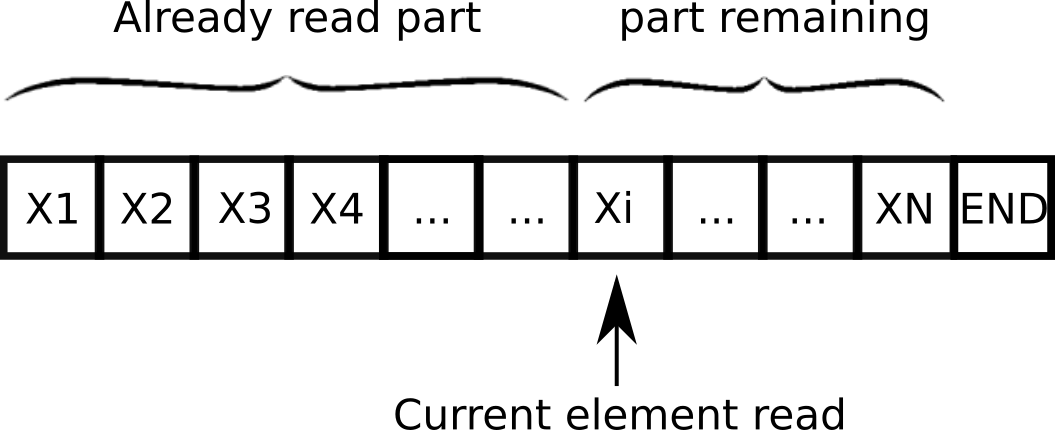
\includegraphics[scale=0.35]{images/sequential_file_principle.png} 
     	%\vspace*{-0.5em}
		%\caption{Floating gate transistor cell}
	\end{figure}		

	\end{frame}
		
	\begin{frame}
		
	Several functions exist to handle files\footnote{The exact naming of the functions may be different depending on the programming language.}:
	
	\begin{itemize}	
	\item {End of file, \textit{eof(file)}: 
		\begin{itemize}
			\item {	returns \textit{True} if the current read element is end of file.}
		\end{itemize}}
	\item {Access first element, \textit{open(file)}:
		\begin{itemize}
			\item{current read element becomes first element.}
		\end{itemize} }
	\item {Read current element, \textit{read(file,val)}: 
		\begin{itemize}
			\item{copy current element in $val$ and go to next element}
		\end{itemize} }
	\item {Create void file, \textit{create(file)}: 
		\begin{itemize}
			\item {create a void content file}
		\end{itemize} }
	\item {Write element, \textit{write(file,val)}:
		\begin{itemize}
			\item {copy $val$ at the end of the file}
			\item {current read element is now last element}		
		\end{itemize}				
	}	
	\end{itemize}		
	  	
	\end{frame}		
		
	\subsection{Reading an element}
	
	\begin{frame}
	
	In order to find the element $val$ in the sequential file, let's do:
	
	\begin{columns}[c]
	\column{.6\textwidth}	
	\begin{center}    
    \scalebox{0.75} {
    %\begin{minipage}
    \begin{algorithm}[H] 
	found=False; c=void\; 
	open(file)\;
    \While{c != val and eof(file) != True} {
		read(file, c)\;
	}
	\If{eof(file) != True} {
		found=True\;
	}    
   	%\caption{InnserSequential search through the array}
	\end{algorithm}	
	%\end{minipage}
	}
	\end{center}	 	
	\column{.4\textwidth}
	\begin{center}
		Complexities:
		\begin{itemize}
			\item {at best: 1}
			\item {at worst: N}
			\item {in average: $\frac{N}{2}$}		
		\end{itemize}			
	\end{center}
	\end{columns}		
	
	\pause
	
	\begin{block}{Notes}
		\begin{itemize}
			\item {$N$ is the number of elements in the file}
			\item {we \textit{cannot} use $\textbf{binary search}$ optimization with sequential files}
		\end{itemize}			
	\end{block}	
	
	\end{frame}
	
	\subsection{Inserting an element}	
			
	\begin{frame}
	
	To insert an element "e" at the position $k$ of a sequential file, let's do:
	
	\begin{columns}[c]
	\column{.5\textwidth}
	\begin{center}    
    \scalebox{0.75} {
    %\begin{minipage}
    \begin{algorithm}[H]
    i=0;possible=False\;
    open(file)\;create(file2)\;
	\While{eof(file) != True and i<k} {
		read(file, c)\;
		write(file2, c)\;
		i=i+1\; 
	}
	\eIf{i==k} {
		write(file2, e)\;
		\While{eof(file) != True}{
			read(file,c)\;
			write(file2,c)\;		
		}
		possible=True\;
	} {
		possible=False\;
	}
	%\caption{InnserSequential search through the array}
	\end{algorithm}	
	%\end{minipage}
	}
	\end{center}	 
	\column{.5\textwidth}
	\begin{center}
	Complexities: 
	\begin{itemize}
		\item {at best: N}
		\item {at worst: N}
		\item {in average: N}
	\end{itemize}		
	\end{center}
	\end{columns}
	
	\end{frame}	
	
	\subsection{Removing an element}
	
	\begin{frame}
	
	To remove the element at the position $k$ of a sequential file, let's do:
	
	\begin{columns}[c]
	\column{.5\textwidth}
	\begin{center}    
    \scalebox{0.75} {
    %\begin{minipage}
    \begin{algorithm}[H]
    i=0;possible=False\;
    open(file)\;create(file2)\;
	\While{eof(file) != True} {
		\eIf{i!=k}{
			read(file, c)\;
			write(file2, c)\;
		} {
			read(file, c)\;
		}
		i=i+1\;		
	}
	\eIf{i<k} {
		possible=False\;
	} {
		possible=True\;
	}
	%\caption{InnserSequential search through the array}
	\end{algorithm}	
	%\end{minipage}
	}
	\end{center}	 
	\column{.5\textwidth}
	\begin{center}
	Complexities: 
	\begin{itemize}
		\item {at best: N}
		\item {at worst: N}
		\item {in average: N}
	\end{itemize}		
	\end{center}
	\end{columns}		
	
	\end{frame}		
				
	\subsection{Summary}			
					
	\begin{frame}
	
	Sequential files...
	
	\begin{itemize}
		\item {...have a \textbf{sequential access} (calling "\textit{read(file, c)}" to "\textit{eof(file)}")}
		\item {...have to be \textbf{rebuilt in case of updates} (insertions, or deletions)} 	
		\item {...have \textbf{implemented functions} to access elements}
		\item {...can be \textbf{read from mass-storage memory}}
	\end{itemize}		
	
	\pause	
	
	\begin{alertblock}{Things to keep in mind}
	\begin{itemize}
	\item{\textbf{Not optimized for fast accesses and updates}}
	\item{More a \textbf{long term data storing structure} (in mass-storage memory)}
	\item{Algorithm \textbf{costs are proportional to the size} of the file}
	\end{itemize}
	\end{alertblock}		
	
	\end{frame}
	
	\section{Linked data structure - Linked-list}	
	\subsection{Properties}	
		
	\begin{frame}
	
	\begin{exampleblock}{Linked?}
	Because each of its element contains the address to go to the next element\footnotemark
	\end{exampleblock}
	
	\begin{figure}
		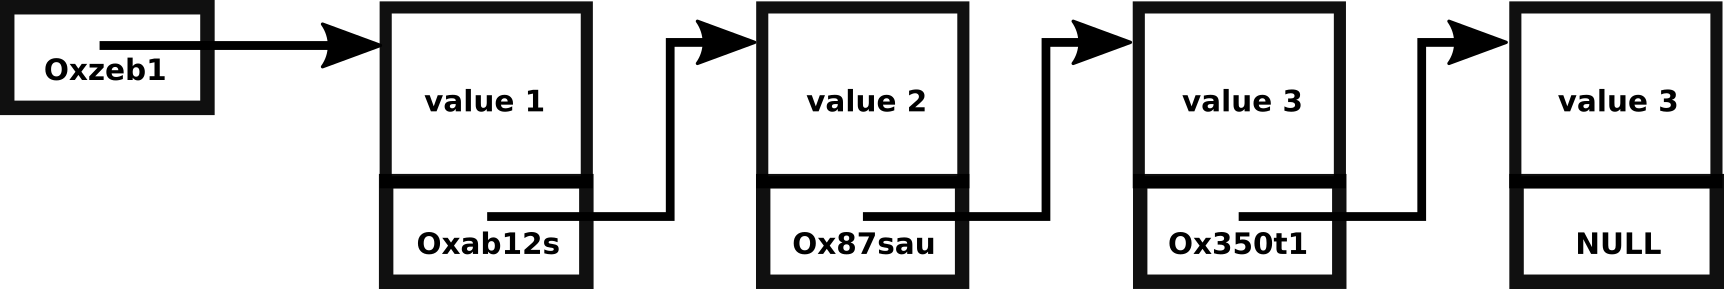
\includegraphics[scale=0.25]{images/linked_list_01.png} 
     	%\vspace*{-0.5em}
		%\caption{Floating gate transistor cell}
	\end{figure}	
	
	Properties:
	
	\begin{itemize}
		\item {A linked-list is \textbf{NOT contiguous in memory}}
		\item {The memory for each \textbf{new element is dynamically allocated}}	
		\item {Like arrays, we can allocate $N$ elements when creating the list}
	\end{itemize}		
		
	\footnotetext{Note that the first "element" only contains an address, the last element contains the NULL address.}
		
	\end{frame}
	
	\subsection{Searching an element}	
	
	\begin{frame}
	
	In order to search an element "e" in a linked-list, let's do\footnote{Accessing the address of an element $p$: $p.address$, and accessing the value: $p.value$.}:
	
	\vspace*{1em}	
	
	\begin{columns}[c]
	\column{.55\textwidth}
	\begin{center}    
    \scalebox{0.75} {
    %\begin{minipage}
    \begin{algorithm}[H]
    p=List.address\;
    \While{p != NULL and p.value != e} {
		p = p.address\;
	}
	%\caption{InnserSequential search through the array}
	\end{algorithm}	
	%\end{minipage}
	}
	\end{center}	 
	\column{.45\textwidth}
	\begin{center}
	Complexities: 
	\begin{itemize}
		\item {at best: 1}
		\item {at worst: N}
		\item {in average: $\frac{N}{2}$}
	\end{itemize}		
	\end{center}
	\end{columns}		
	
	\vspace*{1em}	
	
	\pause	
	
	\begin{block}{Notes}
	\begin{itemize}
		\item {Traversing the linked-list is just fetching the next address until the NULL pointer}
		\item {$N$ is the number of elements in the linked-list}
	\end{itemize}
	\end{block}	

	\end{frame}
	
	\subsection{Inserting an element}
	
	\begin{frame}
	
	The easiest way to insert a new element is \textbf{at the end} of the linked-list:
	
	\begin{columns}[c]
	\column{.5\textwidth}
	\begin{center}    
    \scalebox{0.75} {
    %\begin{minipage}
    \begin{algorithm}[H]
    create(new\_element)\;
  	\vspace*{1em}
    //Search part below \\  
    p=List.address\;
    \While{p != NULL} {
		p = p.address\;
	}
	\vspace*{1em}
	//Insert part below \\ 
    p.address=get\_address(new\_element)\;
   	%\caption{InnserSequential search through the array}
	\end{algorithm}	
	%\end{minipage}
	}
	\end{center}
	\column{.5\textwidth}
	\begin{center}
	\begin{itemize}
		\item {Complexity search part: N}
		\item {Complexity insert part: 1}
	\end{itemize}	
	\end{center}
	\end{columns}	
	
	\end{frame}	
	
	\begin{frame}
	
	You can also insert a new element \textbf{in the linked-list} (ex: after $k$ elements):
	
	\begin{columns}[c]
	\column{.5\textwidth}
	\begin{center}    
    \scalebox{0.75} {
    %\begin{minipage}
    \begin{algorithm}[H]
    create(new\_element)\;
  	\vspace*{1em}
    //Search part below \\
    i=0\;  
    p=List.address\;
    \While{p != NULL and i < k} {
		p = p.address\;
		i=i+1\;
	}
	\vspace*{1em}
	//Insert part below \\ 
	new\_element.address=p.address\;
    p.address=get\_address(new\_element)\;
   	%\caption{InnserSequential search through the array}
	\end{algorithm}	
	%\end{minipage}
	}
	\end{center}
	\column{.5\textwidth}
	\begin{center}
	\begin{itemize}
		\item {Complexity search part: $O(N)$}
		\item {Complexity insert part: 1}
	\end{itemize}	
	\end{center}
	\end{columns}	
		
	\pause
	
	\begin{block}{Note}
	If you know the address after which you want to add an element: complexity = $O(1)$
	\end{block}		
		
	
	\end{frame}
	
	\subsection{Removing an element}	
	
	\begin{frame}	
	Removing an element with value $e$ is \textbf{swapping addresses}:
	
	\begin{columns}[c]
	\column{.50\textwidth}
	\begin{center}    
    \scalebox{0.7} {
    %\begin{minipage}
    \begin{algorithm}[H]
    \vspace*{1em}
    old\_address=NULL\;
    \vspace*{1em}
    //Search part below \\
    p=List.address\;
    \If{List.address.value != e} {  
     	\While{p.address != NULL and p.address.value != e} {
    	   	p=p.address\;
		}
	}
	\vspace*{1em}
	//Remove part below \\ 
	\If{p != NULL} {
		old\_address = p\;
		\eIf{p.address != NULL} {
			p = p.address.address\;
		} {
			p = NULL\;
		}
		delete(old\_address)\;    	
    }
   	%\caption{InnserSequential search through the array}
	\end{algorithm}	
	%\end{minipage}
	}
	\end{center}
	\column{.50\textwidth}
	\begin{center}
	\begin{itemize}
		\item {Complexity search part: $O(N)$}
		\item {Complexity remove part: 1}
	\end{itemize}	
	\end{center}
	\end{columns}	
	
	\end{frame}
	
	\subsection{Summary}
	
	\begin{frame}
		Linked-lists...
		
		\begin{itemize}
		\item {...offer \textbf{more memory flexibility}}
		\item {...allow \textbf{fast element insertions}:
			\begin{itemize}
				\item {no need to allocate $N+1$ memory cells}
				\item {no need to copy $N$ previous cells}
			\end{itemize}		
		}
		\item {...allow \textbf{fast element deletions} (same as above)}
		\item {...can \textbf{only be accessed sequentially} (following the addresses ...)}
		\item {...are \textbf{slower to traverse than arrays} (memory is not contiguous)}
		\end{itemize}
	
	\end{frame}	
	
		
	\section{Abstract data-structure - Stacks}
	\subsection{Properties}
	
	\begin{frame}
			
	\begin{exampleblock}{Abstract?}
		A stack is said \textit{abstract} because:
		\begin{itemize}
			\item {It is \textbf{defined by its behavior}, not its memory management}
			\item {It can \textbf{be based on \textit{arrays} or \textit{linked-list}}}
		\end{itemize}
	\end{exampleblock}
	
	\vspace*{1em}
		
	Properties:
	
	\begin{itemize}
	\item {A new \textbf{inserted element takes the first position}\footnotemark[6]}
	\item {\textbf{Reading the stack = reading the first position}\footnotemark[6]}	
	\item {The \textbf{read element is also removed} from the stack\footnotemark[6]...}
	\end{itemize}
	
	\footnotetext[6]{This is the \textit{LIFO} principle: Last In First Out.}	
	
	\end{frame}
	
	\subsection{Insert and read elements}	
	
	\begin{frame}

	\begin{columns}[c]
	\column{.45\textwidth}
	\begin{center}  
	Array-based stack:
	\scalebox{0.65} {
    %\begin{minipage}
    \begin{algorithm}[H]
    \SetAlgoLined
	\SetKwProg{Fn}{Function}{ is}{end}
	\vspace*{1em}
	level=0\;
	allocate\_memory(Array, N)\;
	\vspace*{1em}
	// Insert stack method \\    
    \Fn{push(value)}{    
		\If{level < N} {
			level = level+1\;
			Array[level] = value;
		}
	}  
    \vspace*{1em}
    // Read stack method\\
    \Fn{pop()}{    	
    	\If{level > 0} {
    		level=level-1\;
    		return Array[level]\;
    	}    
    }  
   	%\caption{InnserSequential search through the array}
	\end{algorithm}	
	%\end{minipage}
	}
	\end{center}
	\column{.55\textwidth}	
	\begin{center}   
	Linked-list based stack:
	\scalebox{0.65} {
    %\begin{minipage}
    \begin{algorithm}[H]
    \SetAlgoLined
	\SetKwProg{Fn}{Function}{ is}{end}
	\vspace*{1em}	
	create\_list(List)\;
	\vspace*{1em}
	// Insert stack method \\    
    \Fn{push(value)}{
    	create\_element(element, value)\;
		old\_address=List.address\;
		List.address=element\;
		element.address=old\_address\;		
	}  
    \vspace*{1em}
    // Read stack method\\
    \Fn{pop()}{
    	\If{List.address != NULL} {
    		p = List.address\;
    		val = p.value\;
    		delete(p)\;
    		return val\;
    	}
    }  
   	%\caption{InnserSequential search through the array}
	\end{algorithm}
	}
    \end{center}
	\end{columns}	
	
	\begin{block}{Common function naming}
	\textit{push}: inserts element in stack, \textit{pop}: read the stack.
	\end{block}	
	
	\end{frame}		
	
	\subsection{Summary}
	\begin{frame}
	Stacks...
	
	\begin{itemize}
	\item {...help organize data in terms of insertions and deletions: 
		\begin{itemize}			
			\item {it \textbf{conserves the order of insertion}}
			\item {you can \textbf{easily reverse back}}
		\end{itemize}
	}
	\item {...automatically \textbf{remove the last read element}}
	\end{itemize}
	
	\vspace*{1em}
			
	\begin{block}{Example of usage}
	The undo mechanism (CTR+Z) in text editors uses a stack.	
	\end{block}		
		
	\end{frame}	
		
	\section{Queues}
	
	\subsection{Properties}
	
	\begin{frame}
	
	\begin{exampleblock}{What's different this time?}
	Queues are also \textit{abstract} BUT are based on the \textit{FIFO}\footnotemark[7] principle	
	\end{exampleblock}	
	
	\vspace*{1em}
	
	Properties:
	
	\begin{itemize}
	\item {A new \textbf{inserted element takes the first position}\footnotemark[6]}
	\item {\textbf{Reading the queue = reading the \textit{last} position}\footnotemark[6]}	
	\item {The \textbf{read element is also removed} from the queue\footnotemark[6]...}
	\end{itemize}
	
	\footnotetext[7]{FIFO: First In First Out (see that as a sort of \textit{waiting line})}	
	
	\end{frame}				
		
	\begin{frame}
	
	\begin{figure}
		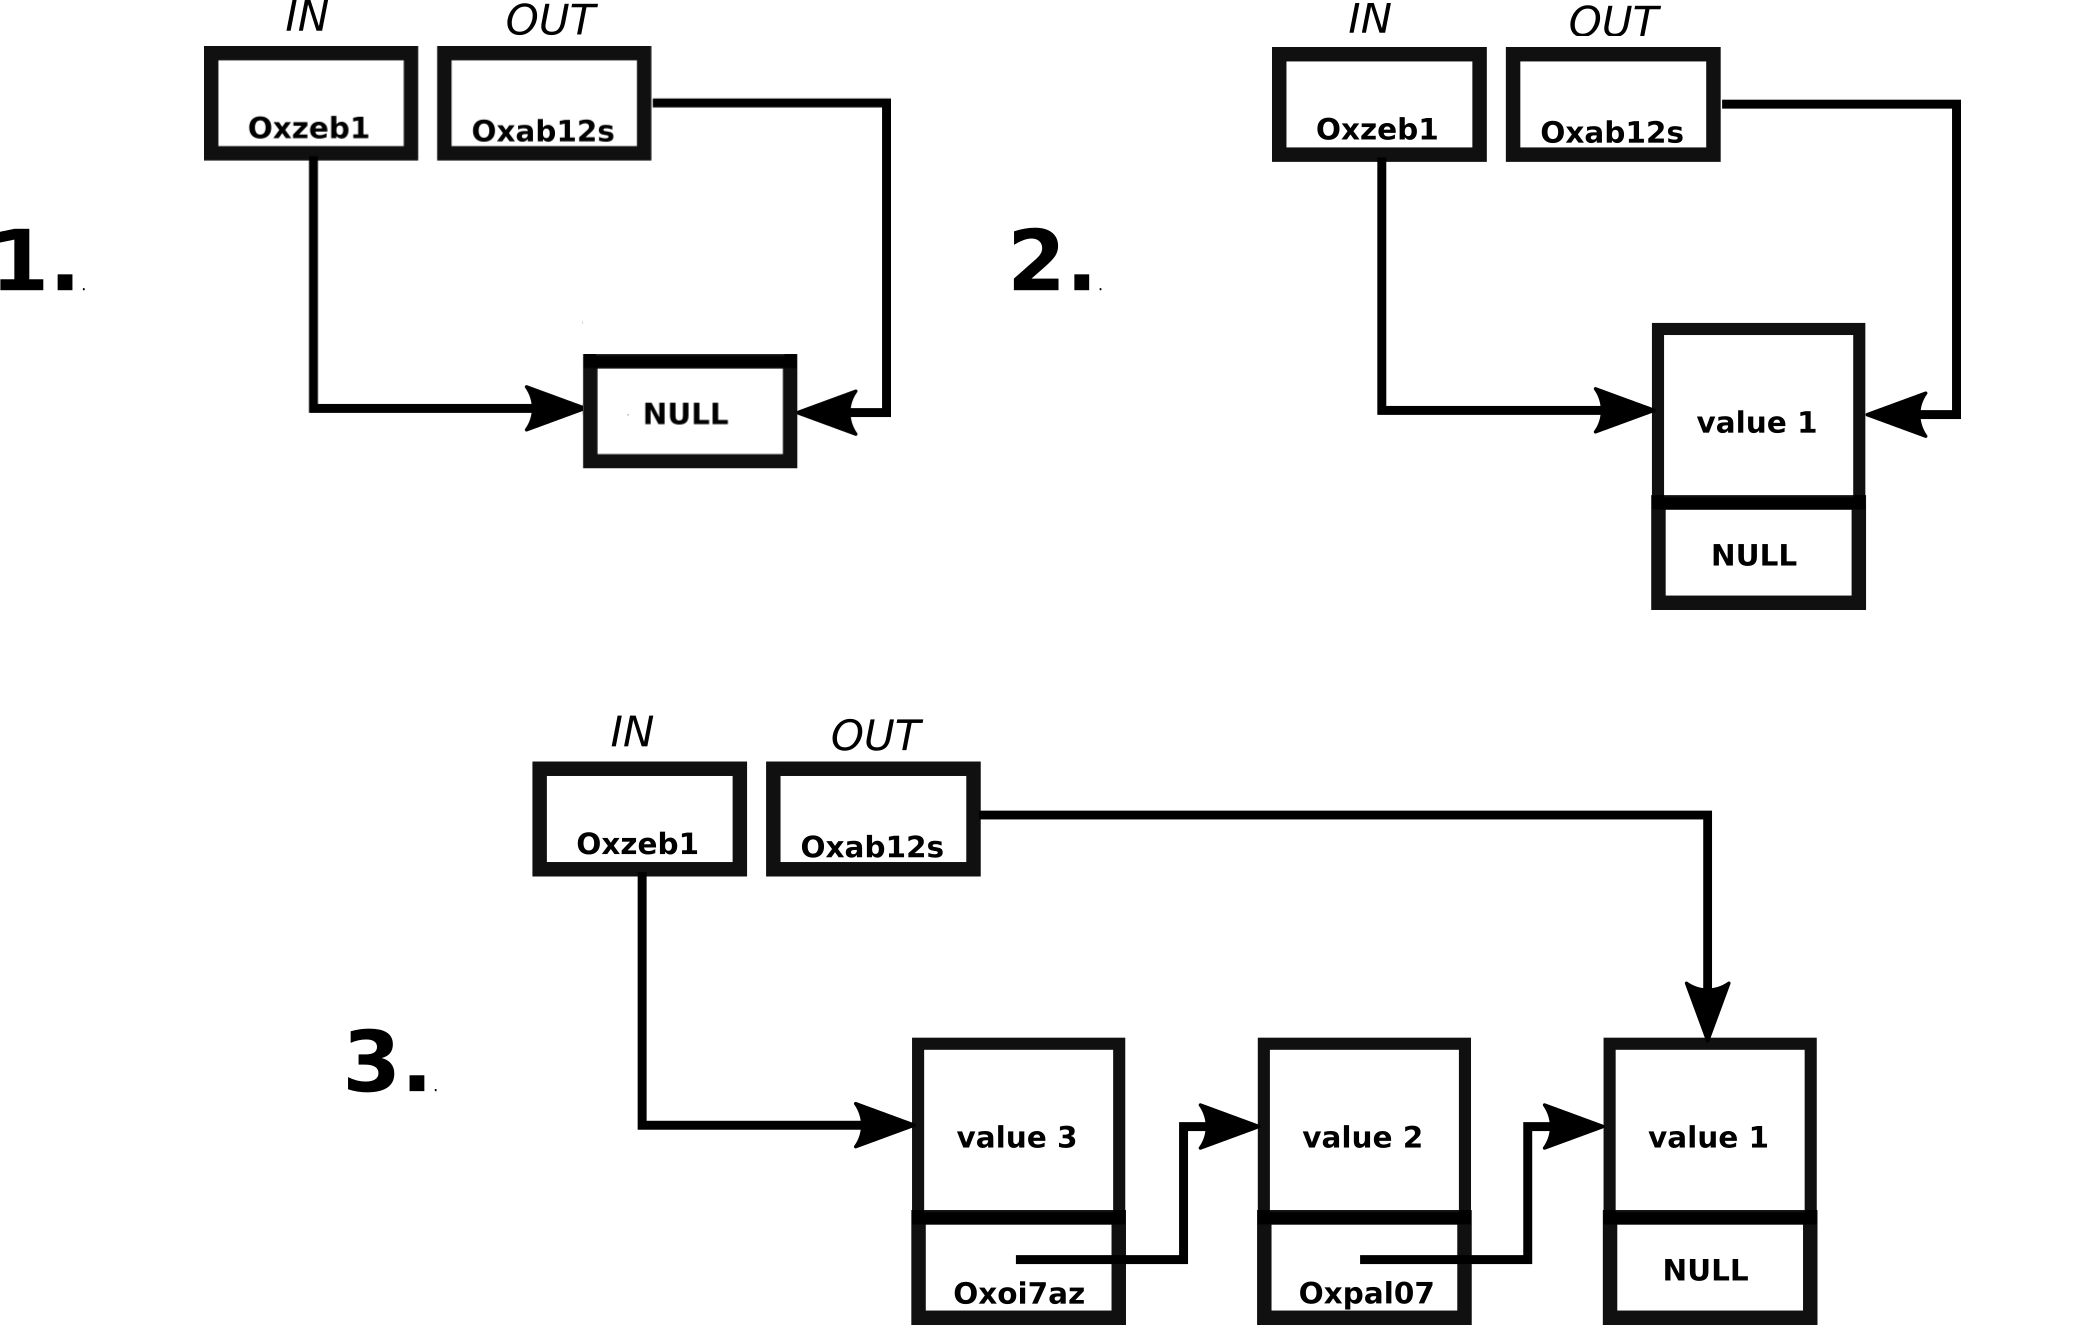
\includegraphics[scale=0.23]{images/queue_example.png} 
	\end{figure}	
	
	\begin{enumerate}
		\item {Initial state: both \textit{in} and \textit{out} addresses point to NULL\footnotemark[8]}
		\item {Inserting element: \textit{in} points to new first element\footnotemark[8]}
		\item {Inserting elements: \textit{in} points to new first element, \textit{out} points to last\footnotemark[8]}	
	\end{enumerate}		
		
	\footnotetext[8]{In this example, we illustrated a linked-list based queue.}		
		
	\end{frame}		
	
	\subsection{Insert and read elements}	
	
	\begin{frame}

	\begin{columns}[c]
	\column{.45\textwidth}
	\begin{center}  
	Array-based queue:
	\scalebox{0.55} {
    %\begin{minipage}
    \begin{algorithm}[H]
    \SetAlgoLined
	\SetKwProg{Fn}{Function}{ is}{end}
	\vspace*{1em}
	number=0;first=0;last=0\;
	allocate\_memory(Array, N)\;
	\vspace*{1em}
	// Insert queue method \\    
    \Fn{enqueue(value)}{
    	\If{number < N} {
			number = number+1\;
			Array[last] = value\;
			last = (last+1) \% N\;
		}
	}  
    \vspace*{1em}
    // Read queue method\\
    \Fn{dequeue()}{
    	\If{number > 0} {
    		number=number-1\;
    		r = Array[first]\;
    		first = (first+1) \% N\;
    		return r\;
    	}    
    }  
   	%\caption{InnserSequential search through the array}
	\end{algorithm}	
	%\end{minipage}
	}
	\end{center}
	\column{.55\textwidth}	
	\begin{center}   
	Linked-list based queue:
	\scalebox{0.55} {
    %\begin{minipage}
    \begin{algorithm}[H]
    \SetAlgoLined
	\SetKwProg{Fn}{Function}{ is}{end}
	\vspace*{1em}	
	In=NULL;Out=NULL\;
	\vspace*{1em}
	// Insert queue method \\    
    \Fn{enqueue(value)}{
    	create\_element(element, value)\;
		\eIf{Out == NULL} {
			Out = element\;
		} {
			element.address = In\;
		}								
		In = element\;
	}  
    \vspace*{1em}
    // Read queue method\\
    \Fn{dequeue()}{
    	\If{In != NULL} {
    		p = In\;
			In = In.address\;
			val =  p.value\;    		
    		delete(p)\;
    		return val\;
    	}
    }  
   	%\caption{InnserSequential search through the array}
	\end{algorithm}
	}
    \end{center}
	\end{columns}	
	
	\begin{block}{Common function naming}
	\textit{enqueue}: inserts element in queue, \textit{dequeue}: read the queue.
	\end{block}	
	
	\end{frame}			
	
	\subsection{Summary}	
	
	\begin{frame}
	
	Queues...
	
	\begin{itemize}
		\item {...help organize data in terms of insertions: 
		\begin{itemize}			
			\item {first element \textit{inserted} become first element \textit{out} (\textbf{FIFO})}
			\item {see that as a \textit{waiting list}}
		\end{itemize}
	}
	\item {...automatically \textbf{remove the last read element}}
	\item {...are \textbf{useful for asynchronous data distribution} (buffering):
		\begin{itemize}
			\item {newly added data is stored in the queue (as temporary storage)}
			\item {when needed, data is extracted from the queue}
		\end{itemize}			
	} 
	\end{itemize}
	
	\vspace*{1em}
			
	\begin{figure}
		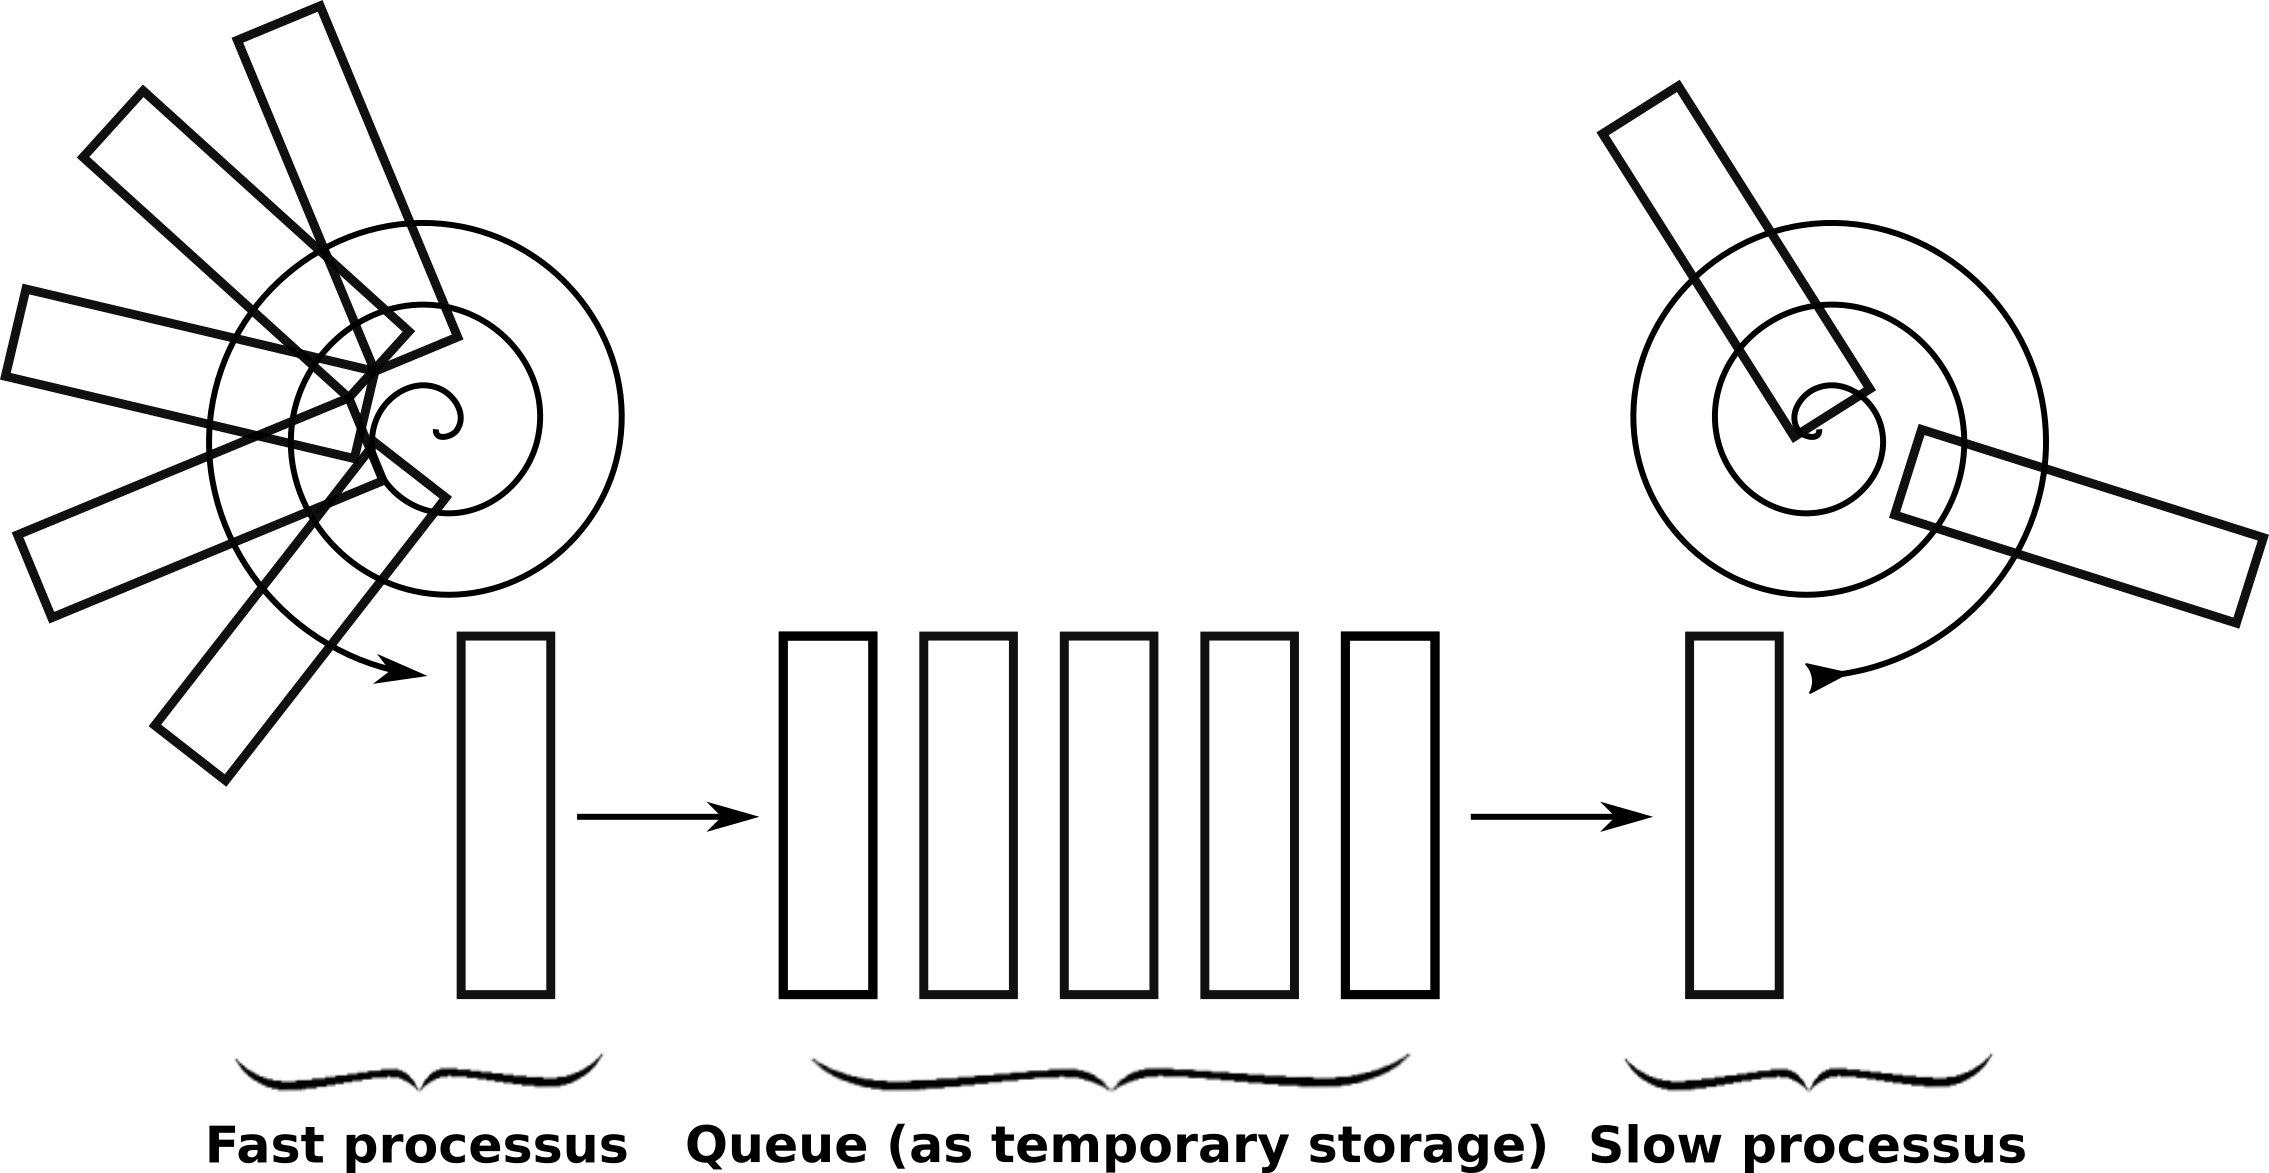
\includegraphics[scale=0.2]{images/queue_example_usage.png} 
     	%\vspace*{-0.5em}
		%\caption{Floating gate transistor cell}
	\end{figure}	
			
	\end{frame}

	\section{Hash-table and hash function}
	\subsection{Properties}
				
	\begin{frame}
	\begin{block}{Hash function?}
	A hash function takes a \textbf{key in input} and \textbf{transforms it into an index}
	\end{block}
	
	\begin{figure}
		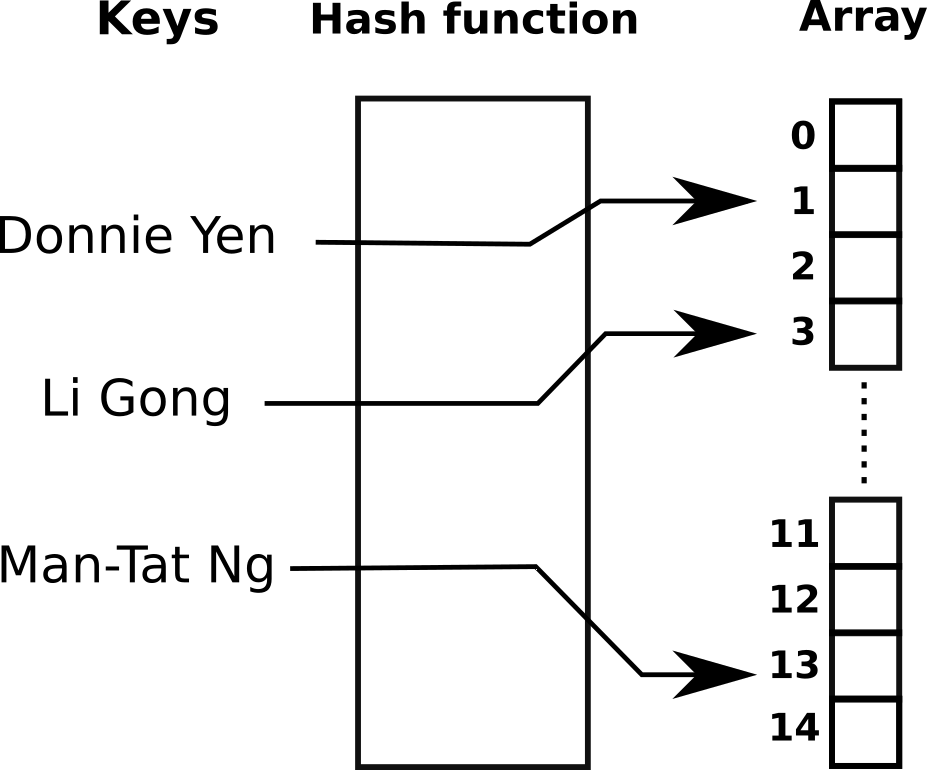
\includegraphics[scale=0.28]{images/hash.png} 
     	%\vspace*{-0.5em}
		%\caption{Floating gate transistor cell}
	\end{figure}		
	
	\vspace*{-1.5em}	
	
	Properties:
	
	\begin{itemize}
		\item {An hash function is an essential part of a hash-based data structure}
		\item {Hash-based data structures\footnote{Also known as \textit{hash table} (or \textit{hash map})} allow direct data access (through \textit{keys})}
		\item {Keys can be of various nature (words, sentences, numbers, and so on)}
	\end{itemize}		
		
	
	\end{frame}
	
	\subsection{Choosing the right hash function}	
	
	\begin{frame}
	
	The ideal \textit{hash function} should be \textit{bijective}\footnotemark[9]: 	
	
	\begin{figure}
		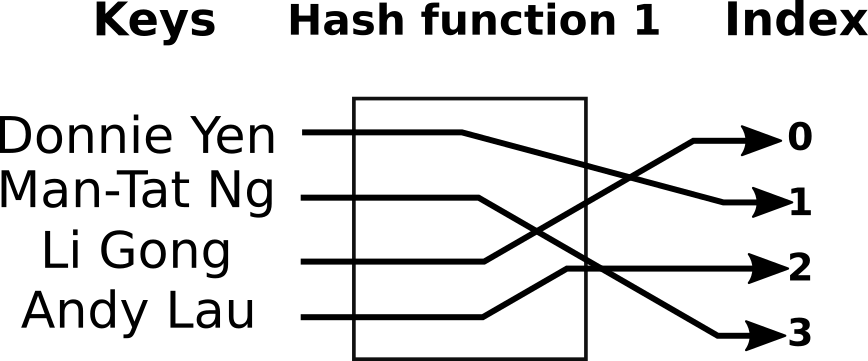
\includegraphics[scale=0.25]{images/hash_01.png} 
     	%\vspace*{-0.5em}
		%\caption{Floating gate transistor cell}
	\end{figure}	
	
	In reality most \textit{hash functions}	are not \textit{bijective}, there are \textbf{collisions}:
	
	\begin{figure}
		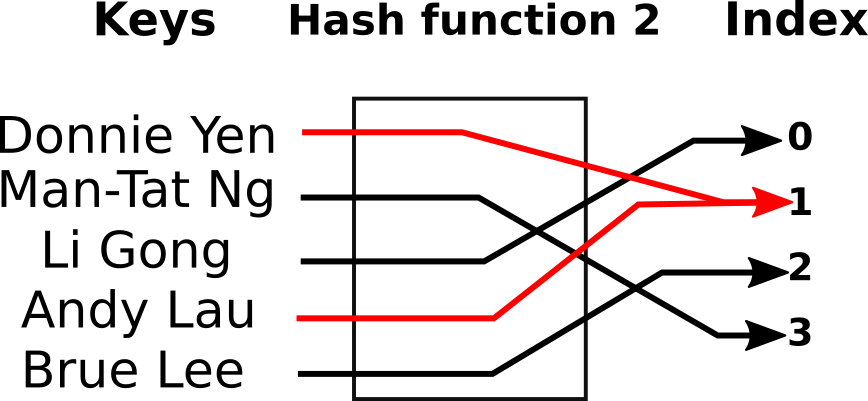
\includegraphics[scale=0.25]{images/hash_02.png} 
     	%\vspace*{-0.5em}
		%\caption{Floating gate transistor cell}
	\end{figure}	
		
	\footnotetext[9]{bijective = for each input \textit{one and only one} output associated}	
	
	\begin{exampleblock}{What criteria for a good hash function?}
	\begin{itemize}
	\item {Have the \textbf{fewest possible collisions}}
	\item {\textbf{Uniformly} distribute the indexes (spreading the data along the array)}	
	\end{itemize}		
	\end{exampleblock}	
	
	\end{frame}	
		
	\begin{frame}
	
	A good example of hash function is the $h_1$ function:
	
	\vspace*{1em}	
	
	\scalebox{0.8} {
	$h_1(key) = (f(key[0]) + f(key[1])\times 26 + f(key[2])\times 26^2  + ... + f(key[k])\times 26^k)) \% N$
	}
	
	\vspace*{1em}
	
	Where the $f$ function gives the alphabet number, ex: $f(c)==2$.
	
	\vspace*{1em}	
	
	Example (let's say $N=100000$):
	
	\vspace*{1em}
	
	\scalebox{0.8}{
	$h_1(hello)=(f(h)+f(e)\times 26+f(l)\times 26^2 +f(l)\times 26^3+f(o)\times 26^4)\%N$ 
	}
	\vspace*{0.1em}
	
	\scalebox{0.8}{
	$h_1(hello)=(7+4*26+11*26^2+11*26^3+14*26^4)\%100000$ 
	}
	\vspace*{0.1em}
	
	\scalebox{0.8}{
	$h_1(hello)=98547$
	}
	
	\vspace*{1em}	
	
	\begin{block}{Note}
	$N$ is the maximum number of elements that can be stored in the hash-table 
	\end{block}	
	
	\end{frame}		
		
	\subsection{Handling collisions}
	\begin{frame}
	
	Although quite rares, collisions can be managed using:
	
	\vspace*{1em}	
	
	\begin{itemize}
	\item {\textit{external chaining}
		\begin{itemize}
		\item {interesting if we \textbf{don't know how many keys we have to handle}}
		\item {interesting if we have \textbf{lots of insertions/deletions}}
		\item {but, likely to consume a \textbf{lot more memory}}			
		\end{itemize}			
	}	
	\item {or \textit{internal chaining}
		\begin{itemize}
		\item {interesting if we \textbf{KNOW how many keys we have to handle} ($<N$)}
		\item {but, if \textbf{many collisions to handle = slower} than external chaining}
		\item {is a \textbf{lighter structure} (consuming less memory)} 
		\end{itemize}			
	}	
	\end{itemize}		
		
	\end{frame}
	
	\begin{frame}
	External chaining:	
	
	\begin{figure}
		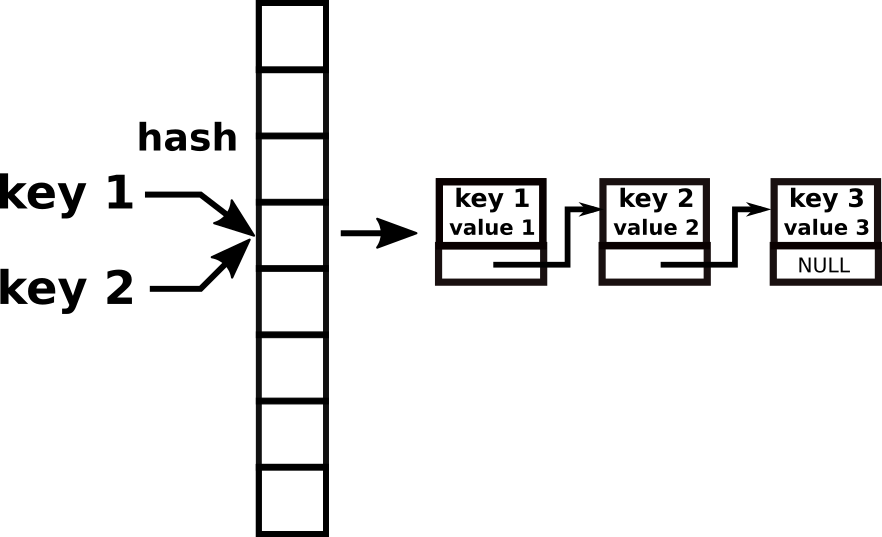
\includegraphics[scale=0.25]{images/collisions_external.png} 
     	%\vspace*{-0.5em}
		%\caption{Floating gate transistor cell}
	\end{figure}	
	
	\vspace*{-2em}	
	
	\begin{itemize}
		\item {Insertion:
			\begin{itemize}
			\item {if void, we \textbf{insert the first linked-list element}}
			\item {if no void (collision occurred), we \textbf{add a linked-list element}}
			\end{itemize}							
		}
		\item {Reading:
			\begin{itemize}
			\item {we \textbf{sequentially search} in the linked-list}			
			\item {finding and element \textbf{with same key}: we found the right element}
			\end{itemize}
		}	
	\end{itemize}		
		
	\end{frame}	

	\begin{frame}	
	
	Internal chaining:	
	
	\begin{figure}
		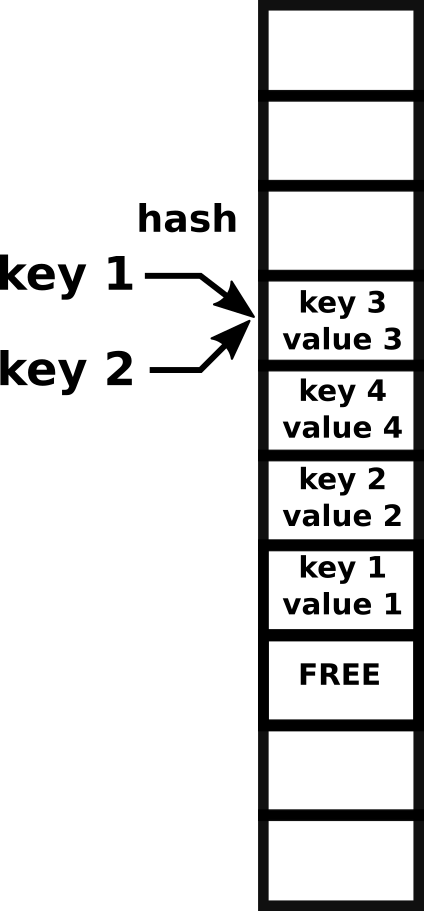
\includegraphics[scale=0.25]{images/collisions_internal.png} 
     	%\vspace*{-0.5em}
		%\caption{Floating gate transistor cell}
	\end{figure}		
	
	\vspace*{-2em}
	
	\begin{itemize}
		\item {Insertion:
			\begin{itemize}
				\item {if void, we \textbf{insert the element}}
				\item {if it collides, we \textbf{search for next FREE element and insert}} 
			\end{itemize}				
		}
		\item {Reading:
			\begin{itemize}
				\item {if we have the \textbf{same key: we take the value}}
				\item {if not, we \textbf{search in the next elements}}
			\end{itemize}		
		}
	\end{itemize}		
	
	\end{frame}

	\subsection{Complexities}
	
	\begin{frame}
	
	Complexities for accessing a hash-table element (insert, read, delete):
	
	\vspace*{1em}	
	
	\begin{center}
		
	\begin{tabular}{|c|c|c|}
	\hline
	\textbf{Complexities} & \textbf{At best} & \textbf{At worst} \\ \hline 
	No collision management & 1 & 1 \\ \hline
	External chaining & 1 & N \\ \hline
	Internal chaining & 1 & N \\ \hline
	\end{tabular}
	\end{center}		
	
	\end{frame}

	\subsection{Summary}
	
	\begin{frame}
	
	Hash-tables...	
	
	\begin{itemize}
		\item {...are \textbf{fast in insertions}, \textbf{reading} and \textbf{deletions}:
			\begin{itemize}
				\item {\textbf{no need to search} in the data structure (if the key is well thought)}
				\item {if \textbf{collisions are rares: complexity near 1}}
				
			\end{itemize}
		}	
		\item {...\textbf{cannot be accessed sequentially}} 
		\item {...are \textbf{difficult to design} (better use default ones):
			\begin{itemize}
				\item {\textbf{bad hash function = more collisions} = slow}
				\item {\textbf{not enough memory ($N$ small) = more collisions} = slow}
			\end{itemize}
		}
	\end{itemize}		
	
	\vspace*{1em}
	
	\begin{block}{Example}
	Hash-table giving the international telephone code knowing the country:
	Hash[china] == 86,
	Hash[france] == 33, hash[germany] == 49
	\end{block}		
			
	\end{frame}	
	
\end{document}